\newpage
\section{Solutions of differential equations}
\subsection{Initial value problems}
Initial value problems are differential equations of the form
\begin{equation}
    \label{eq:ivp}
    \diff{\bv y}{t} = \bv f(\bv y, t),
\end{equation}
where $\bv y$ is a vector, $t$ is the time and $\bf f$ is an arbitrary function together with the initial condition $\bv y(t=0) = \bv y_0$. Note that the equation is always written in the form of a first-order ordinary differential equation. However, differential equation of any order can be re-written as a first order equation by setting the vector $\bv y = (y(t), y'(t), y''(t), \dots)$. For example, a Newton's law of motion, $\ddot x = F/m$ would correspond to $\bv y = (x, \dot x)$ and $\bv f = (\dot x, F/m)$.

These types of equations are usually solved by \emph{time stepping}: given that we know $\bv y(t=0) = \bv y_0$, we calculate $\bv y(\dd t) \approx \bv y(0) + \bv f(\bv y(0), 0)\dd t$; $\bv y(2\dd t) \approx \bv y(\dd t) + \bv f(\bv y(\dd t), \dd t)\dd t$ $\dots$. This time stepping is called the \emph{Euler} method and generally requires a small time step to be accurate and numerically stable.\footnote{Numerical \emph{in}stability is the tendency of an error (i.e., the difference between the true solution and its numerical approximation) to oscillate wildly or grow to infinity.} There are many time stepping schemes that are more accurate and stable than the basic Euler method. The accuracy of the method is often quantified using the big-O notation, i.e., the Euler method is $O(\dd t)$, or a first-order method, which means that if we halve the time step $\dd t$, we also halve the error at every step. Very common are the explicit Runge-Kutta methods, of which the 4-th order version (with accuracy $O(\dd t^4)$) is probably the most common, i.e., if we halve the time step, the error decreases by factor 16.

The fourth-order Runge Kutta (RK4) calculate $y(t + \dd t)$ from $y(t)$ as
\begin{equation}
    \label{eq:RK4}
    y(t + \dd t) = y(t) + \frac{\dd t}{6}\left(k_1 + 2k_2 + 2k_3 + k_4\right),
\end{equation}
where
\begin{equation}
    \begin{aligned}
        k_1 &= f(y_t, t)\\
        k_2 &= f\left(y_t + \frac{1}{2}\dd t k_1, t + \frac{1}{2}\dd t\right)\\
        k_3 &= f\left(y_t + \frac{1}{2}\dd t k_2, t + \frac{1}{2}\dd t\right)\\
        k_4 &= f(y_t + k_3 \dd t, t + \dd t).
    \end{aligned}
\end{equation}
Notice that for each time step, the function $f$ has to be evaluated 4 times, and the calculation is about 4 times slower than the Euler method. There are also time stepping methods which instead of taking 4 times as long, the take-up 4 times as much space (e.g., Adams-Bashforth family of methods) which use the last four steps in the history of $y(t)$ to estimate the next step.

The RK4 method for a problem of type \eqref{eq:ivp} is implemented in \verb|SciPy| in \ls{scipy.integrate.solve_ivp()}. The \ls{solve_ivp()} expects the function $f(t, y)$, which takes the time and state vector and returns the time derivative of the state vector, the initial condition, and the time range where the evolution should be calculated.

The calculation can also watch for \emph{events} -- typically a signal, that a calculation should end. These are functions of time and the state vector which \emph{change sign} when the event occurs. An event can be made terminal (i.e., when even occurs calculation should stop) by simply setting the \ls{terminal} attribute of the function to \ls{True}. Remeber, functions are objects, and we can set their attributes as we please (similarly to \ls{self.attribute = value} when working with classes).

\textbf{Example}: Calculate the ballistic trajectory of a ball kicked under angle of 45$^\circ$ with initial velocities of 3 m/s along both $x$ and $y$ directions. The ballistic trajectory is the trajectory of a projectile thrown in a medium (e.g., air) which exerts nonlinear drag force on the motion of the form
\begin{equation}
    \bv F_d = -\frac{1}{2}A|\bv v|\bv v \rho \mathrm{CD},
\end{equation}
where $\bv v$ is the velocity of the projectile, $A$ is the area of the projectile projected facing the direction of motion, $\rho$ is the density of the medium and CD is the drag coefficient, $\mathrm{CD}\approx0.47$ for a ball.

\textbf{Solution:}
Full code is available in \ls{ivp_ballistic.py}. First, we import necessary modules and define the needed constants
\lstinputlisting[linerange={1-10}]{../example_code/ivp_ballistic.py}

Next we define the function $f$. We take the state vector $\bv x = (x, y, v_x, v_y)$ to represent both the position and velocity vectors. The function must return the time derivative of this 4-component state vector
\lstinputlisting[linerange={12-25}]{../example_code/ivp_ballistic.py}

Next we define the event that will indicate that the ball hit the ground and make it terminal, because we do not want the calculation to continue past this point
\lstinputlisting[linerange={30-34}]{../example_code/ivp_ballistic.py}

Now we have everything we need to calculate the ballistic trajectory. We set the calculation time range to $(0, 10)$, 10 being just arbitrary large time, the calculation will be stopped by the impact event. We also pass additional arguments, the drag coeffecient, through the usual \ls{args=} keyword argument. Finally, we also ask for a \ls{dense_output}, which will return an interpolation object (\ls{solution.sol} below) to represent the solution. This is useful, because \ls{solve_ivp} uses adaptive size of the time step $\dd t$ (i.e., when the derivatives are small and slowly-changing, the time step is bigger), so if we want an evenly sampled solution we have to interpolate it. With the returned solution, we use the time of the event to create an evenly sampled time array and return the interpolated trajectory.

Finally, we calculate the trajectory with and without air resistance and plot. We use slightly non-zero initial condition in the $y$ position to avoid triggering the event in the beginning.
\lstinputlisting[linerange={36-}]{../example_code/ivp_ballistic.py}

% \lstinputlisting{../example_code/ivp_ballistic.py}
\begin{center}
    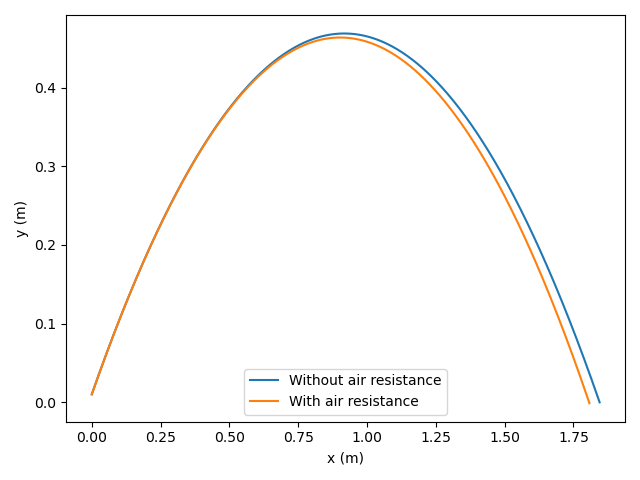
\includegraphics[width=0.6\linewidth]{ballistic.png}
\end{center}

\begin{exercise}
    Simulate the population dynamics of predators and prey (foxes $F$ and rabbits $R$) using the Lotka-Volterra model:
    \begin{equation*}
        \begin{aligned}
            \frac{\dd R}{\dd t} &= aR - bFR\\
            \frac{\dd F}{\dd t} &= dFR - cF
        \end{aligned}
    \end{equation*}
    with $a = 2/3$, $b = 4/3$ and $c = d = 1$. Plot $R(t)$ and $F(t)$ and the trajectory in phase space $R-F$.
\end{exercise}

\begin{exercise}
    Simulate the Lorenz system (the first properly studied example of deterministic chaos) given by equations
    \begin{equation*}
        \begin{aligned}
            \frac{\dd x}{\dd t} &= \sigma (y - x)\\
            \frac{\dd y}{\dd t} &= x(\rho - z) - y\\
            \frac{\dd z}{\dd y} &= xy - \beta z,
        \end{aligned}
    \end{equation*}
    with $\sigma = 10$, $\rho = 28$, and $\beta = 8/3$. Plot the $x$, $y$, $z$ trajectory in 3D space.
\end{exercise}

\begin{syntax}[3D plotting]
Matplotlib supports 3D plotting. On recent versions of matplotlib, a simple 3D plot of a line given by arrays \ls{x}, \ls{y}, and \ls{z} is very simple:
\begin{lstlisting}
fig3d = plt.figure()
ax3d = fig3d.add_subplot(projection='3d')
ax3d.plot(x, y, z, lw=0.5)
\end{lstlisting}
\end{syntax}

\subsection{Boundary value problems}
Boundary value problems are differential equations of the form
\begin{equation}
    \label{eq:bvp}
    F(\bv y, x) = 0
\end{equation}
where $F$ is some function that defines our problem that depends on the unknown function itself and its derivatives, $\bv y$ is the unknown function of $x \in [a,b]$ subject to boundary conditions $B(y_a, y_b) = 0$. Here the unknown function is a function of space, rather than time, and we need to know the solution "everywhere" at once. The numerical algorithms typically start from some initial guess and then iteratively optimize the solution $\bv y$ to fulfill the equation \eqref{eq:bvp} while maintaining the boundary conditions.

Solution of 1D (dimension of $x$) boundary value problems is implemented in \verb|SciPy| in \ls{scipy.integrate.solve_bvp}, which also allows for finding unknown parameters for which the solution can exist (see example below). For multi-dimensional problems, you typically have to use a dedicated package or write your own.

We will solve a simple example of a 1D Schr\"{o}dinger equation:\\
\textbf{Example} Calculate the wave functions and energy levels of a particle in inifinite potential well with additional potential $V(x)$ inside the well.

The states of a quantum particle are described with a stationary Schr\"{o}dinger equation
\begin{equation}
    \label{eq:sch}
    E\psi = -\frac{\hbar^2}{2m}\frac{\dd^2\psi}{\dd x^2} + V(x)\psi,
\end{equation}
where $m$ is the particle mass, $\psi$ is the particle wave function and $E$ is the energy. Calculate in "atomic units", $\hbar = 1$, $m=1$ and potential of the shape shown in Fig.~\ref{fig:potential}, i.e., $V(|x| > 1) = \infty$ and $V(|x| < 0.1) = 10)$ and $V=0$ elsewhere.
\begin{figure}[h!]
    \centering
    \label{fig:potential}
    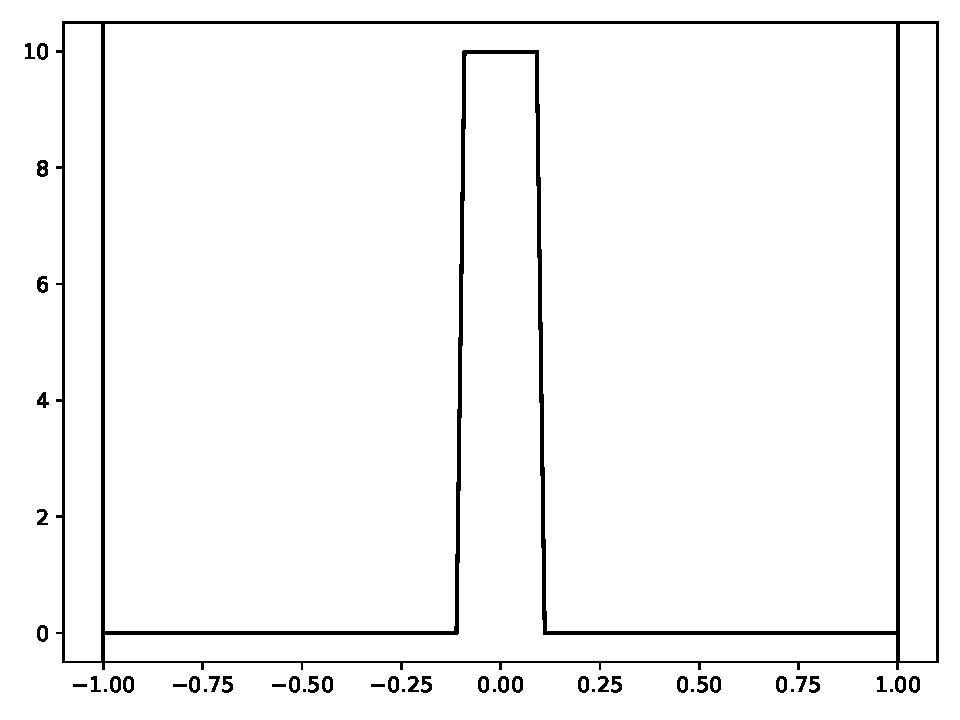
\includegraphics[width=0.5\linewidth]{sch_potential.pdf}
    \caption{Potential for the Schrödinger equation \eqref{eq:sch}.}
\end{figure}

\textbf{Solution:} The full code is available in \ls{bvp_schrodinger.py}. 

Begin by importing everything we need, define the constants \ls{w}, the width of the barrier and \ls{dh} the height of the barrier and the potential function itself. The infinite walls at $x=\pm 1$ will be taken care of by the boundary conditions.
\lstinputlisting[linerange={6-21}]{../example_code/bvp_schrodinger.py}

Next, define the function $F$ from \eqref{eq:bvp}. We rewrite the Schrödinger equation \eqref{eq:sch} to
\begin{equation}
    \frac{\dd^2\psi}{\dd x^2} = 2m(V(x) - E)\psi,
\end{equation}
and the unknown function $\bv y$ is then $(\psi, \dd \psi/\dd x)$. Finally, we also need to find the unknown parameter $E$. The function $F$ can depend on a vector of unknown parameters which \ls{solve_bvp()} finds together with the unknown function. In this case, this is just the energy.
\lstinputlisting[linerange={23-29}]{../example_code/bvp_schrodinger.py}

Next is the function representing the boundary conditions. This is an arbitrary function of the value of the unknown function at the boundaries and unknown parameters which the \ls{solve_bvp} maintain at zero. We have to return a vector of size 2 (i.e., the number of boundaries) + number of unknown parameters. In our case we simply want the wave function to be zero at the infinite wall. The third boundary condition is arbitrary, and its purpose is to simply ensure that the found solution is not identically 0.
\lstinputlisting[linerange={35-36}]{../example_code/bvp_schrodinger.py}
The number in the third condition is arbitrary, because the solution provided by \ls{solve_bvp} is not normalized.

Next we need to create the initial condition, both for the wave function and the energy, for the solver to optimize. Note that the original Schrödinger equation \eqref{eq:sch} has infinitely many solutions. To which solution \ls{solve_bvp()} actually converges is given by this initial condition. First we create the grid, i.e., points in space $x$ which are the argument of the wave function and create a simple estimate of wave function which is zero everywhere and non-zero in one off center point, in order to converge to a solution localized in one half of the potential well. Remember, the full initial condition is the wave function and its gradient, so \ls{y_0} is a 2D array of size 2 $\times$ length of \ls{x}.
\lstinputlisting[linerange={38-50}]{../example_code/bvp_schrodinger.py}

For the energy, we simply use the ground state energy of a particle in a simple infinite potential well.
\lstinputlisting[linerange={53}]{../example_code/bvp_schrodinger.py}

Finally, we have everything we need to call \ls{solve_bvp()}. Physically, the most interesting part is the probability of finding the particle at a position $x$, which is given by $|\psi(x)|^2$, so we plot that. To be exact, we should also normalize the wave function such that $\int |\psi(x)|^2 \dd x = 1$, however, since we are not calculating any quantum mechanical expectation values and are only interested in the shape of the distribution we plot it as it is, together with the potential and found energy.
\lstinputlisting[linerange={56, 65-74}]{../example_code/bvp_schrodinger.py}

\subsection{GPU acceleration}
Certain types of physical problems can be effeciently calculated on graphics cards (GPUs). These are problems which involve many independent calculations which can be run in parallel. A prototypical example is the gravitational $N$-body problem: calculate the motion of $N$ planets with equal masses $m$ that interact with each other via gravity only.

We will consider the 2D case for simplicity of plotting. The total force acting on planet $j = 1\dots N$ is
\begin{equation}
    \bv F_j = Gm^2\sum_{k\neq j}\frac{\bv r_k - \bv r_j}{|\bv r_k - \bv r_j|^3},
\end{equation}
where $G$ is the gravitational constant and $\bv r_k$ are the positions of the planets. The motion of the planet is then given simply by $m\ddot{\bv r_j} = \bv F_j$ and we could use \ls{solve_ivp()} as before. However, this problem becomes more scientifically interesting for large number of planets where \ls{solve_ivp()} would quicktly grind to a halt. Therefore we want to make use of fast GPUs.

The calculation will proceed again in steps: we will keep stored all positions and velocities of the planets. In every step, we will calculate the total force acting on all planets and then update positions and velocities via Euler stepping for simplicity. The calculation involves $N^2$ calculations of forces between planests which are independent of each other. Our goal is to use the GPU tu run these in parallel.

The full code is \verb|example_code/taichi/gravity.py|

\subsubsection{Setting up the environment}
We will be using the \ls{taichi} library to accelerate the computation from within Python, which has the advantage that it is rather simple, looks very much like standard Python code and allows using either GPU or CPU with the same code, so you can still try the code below even if you do not have a dedicated GPU in your computer. Taichi unfortunately requires Python version 3.10, which is most likely not the version you have installed. We do not want to clutter the system with multiple python versions, therefore we will use a \emph{virtual environment} to have an isolated installation of Python with its own version and packages.

The easiest way to manage virtual environments is with the \ls{uv} tool \url{https://docs.astral.sh/uv/getting-started/installation/}. On Windows, run the installation commands in the Windows Powershell.

Once \ls{uv} is installed, create an empty directory, let's call it "gravity", navigate to it in the command line and run
\begin{lstlisting}[language=bash]
uv venv -p 3.10
\end{lstlisting}
which will create the virtual environment with Python version 3.10. You shoud see output that looks similar to
\begin{verbatim}
Using CPython 3.10.16 interpreter at: /usr/bin/python3.10
Creating virtual environment at: .venv
Activate with: source .venv/bin/activate
\end{verbatim}
Activate the virual environment with the command from the last line. Your command line prompt shoud now show the virtual environment, e.g., on my linux machine
\begin{verbatim}
(gravity) emil@nt202 ~/gravity $
\end{verbatim}
This is a blank slate where we need to install all Python libraries we need. We will only need \ls{taichi} and \ls{matplotlib} (and their dependencies), which we can install simply using
\begin{lstlisting}
uv pip install taichi matplotlib
\end{lstlisting}
and now we have everything we need to start writing and running taichi code. However, we have to have the environment activated, otherwise we are using system-wide python which is not aware of the taichi library.

\subsubsection{Testing the installation}
TODO

\subsubsection{GPU Kernels}
Taichi allows us to offload specific functions to run on the GPU. These functions are handled differently from the rest of the Python code and are called \emph{kernels}. We will write two kernels, one for calculating the forces and one for the Euler stepping. We will store the data in numpy arrays -- this is not the fastest way (taichi can use memory more effeciently, see the taichi documentation for a more optimized version), but it is the simplest.

We import taichi and as it to use a GPU is possible using
\begin{lstlisting}
import taichi as ti
ti.init(ti.gpu)
\end{lstlisting}
This will use, in order of precedence, NVIDIA CUDA, Vulkan on AMD GPUs or the CPU.

The Euler stepping kernel looks like this
\lstinputlisting[linerange={49-59}]{../example_code/taichi/gravity.py}
We indicate that the function is a kernel using the \ls{ti.kernel} decorator. The function takes four arguments -- the positions of the planets \ls{rs}, the velocities \ls{vel} and accelerations \ls{acc}, which are numpy arrays of 64 bit floats of shape \ls{(N,2)} ($N$ planets and two coordinates) and the time step \ls{dt} which is a simple float.

Inside, the function look rather ordinary, however it does run inside the GPU and the outer-most for loop is in fact not a loop but iterations are executed in parallel as much as possible. There are some restrictions -- for example, you are not allowed to \ls{break} out of the outermost loop. The inner loop (\ls{for k in range(2)}) runs as an ordinary sequential for loop. We do not return anything, but rather modify the input arrays.

A more interesting kernel is the calculation of accelerations (or forces), which looks like this
\lstinputlisting[linerange={14-46}]{../example_code/taichi/gravity.py}

Our problem is relatively simple, so-called \emph{embarrassingly parallel}\footnote{This is an actual term used in the computer science.} because the calculations are entirely independet of each other. GPUs are capable of running many task in parallel quickly because they do not allow for synchronisation (or only in a very limited form). This means, that despite running many things in parallel, we do not have any mechanism similar to \ls{Lock()} from multithreading. Therefore, if the iterations of the loop depend on each other, avoiding race conditions becomes somewhat more complicated. For example, imagine some planets are made of matter and some of anti-matter and if they get too close to each other they annihilate. We could implement this this for example as
\begin{lstlisting}
for j in range(N):
    for k in range(N):
        if planet_is_alive(j) and planet_is_alive(k):
            if distance(j,k) < annihilation_distance:
                annihilate(j,k)
\end{lstlisting}
This would be OK if the loops are sequential. However, when the outermost loop runs in parallel, we could get to a situation where we have palents $j=1$ (matter) and $k=2, 3$ (anti-matter) which are all close to each other. Since the check on line 3 might be using old data, we could end up running both \ls{annihilate(1,2)} and \ls{annihilate(1,3)} and thus increasing the ratio of matter to anti-matter in the universe.

\subsubsection{Using the kernels}
To represent the state of the simulation -- the positions and velocities of the planets and the time we will use a simple class. As an initial condition we will random positions in 2D with normal distribution around origin and solid body rotation for velocities with some initial angular velocity. The class will have only two methods, which call the two kernels we wrote above,
\lstinputlisting[linerange={61-88}]{../example_code/taichi/gravity.py}

Finally, we create a simulations with 5000 planets, plot a real-time animation using matplotlib and periodically save a picture
\lstinputlisting[linerange={91-130}]{../example_code/taichi/gravity.py}

After about a minute of runtime on Intel Core i7-7700 CPU (a fairly old CPU) the initial gaussian distribution of the planets develops some interesting structure
\begin{center}
    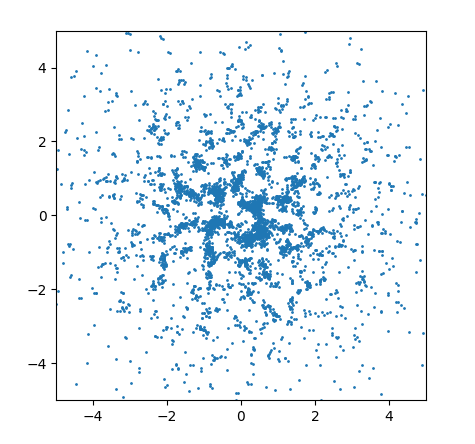
\includegraphics[width=0.5\linewidth]{gravity.png}
\end{center}
